% !TeX root = main.tex

\hypertarget{defining-the-derivative}{%
\section{Defining the Derivative}\label{defining-the-derivative}}

\hypertarget{difference-quotient}{%
\subsection{Difference Quotient}\label{difference-quotient}}

Let \(f\) be a function defined on an interval \(I\) containing \(a\).
If \(x\neq a\) is in \(I\), then the \emph{difference quotient.} is \[
Q=\frac{f(x)-f(a)}{x-a}.
\] If \(h\neq 0\) is chosen so that \(a+h\) is in \(I\), then \[
Q=\frac{f(a+h)-f(a)}{a+h-a}=\frac{f(a+h)-f(a)}{h}
\] is a difference quotient with increment \(h\).

The slope of a tangent line is the limit of a difference quotient \[
m_{t a n}=\lim\limits_{x \to a} \frac{f(x)-f(a)}{x-a} .
\] Equivalently, \[
m_{\tan }=\lim\limits_{h \to 0} \frac{f(a+h)-f(a)}{h}
\]

\begin{figure}[h!]
\centering
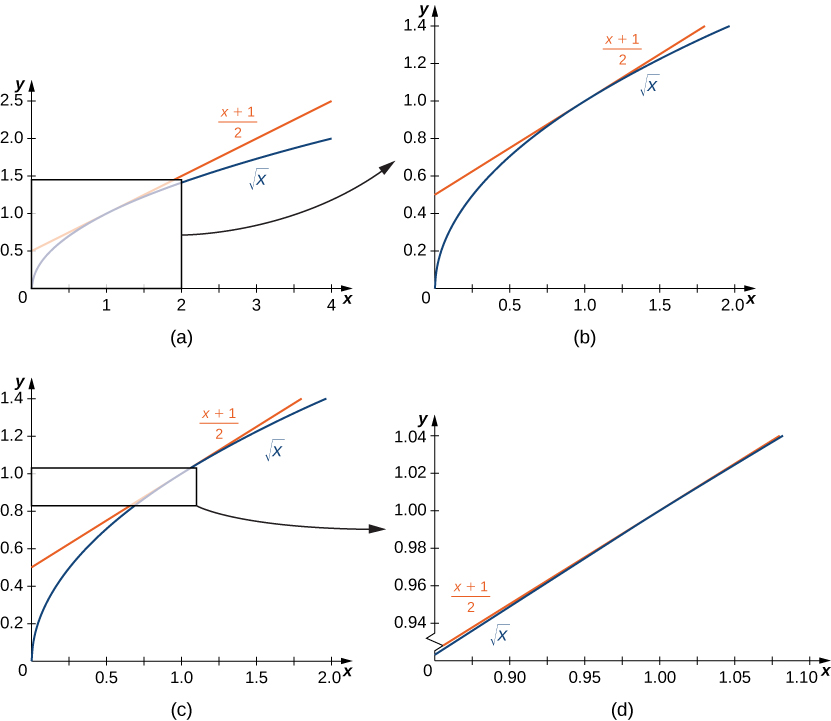
\includegraphics[width=\textwidth]{img/locally-linear.jpeg}
\par Smooth curves are locally linear
\end{figure}

\begin{example}
  Find the equation of the line tangent to the graph of  $f(x)=x^2$  at $x=3$.
\end{example}
\vspace*{6\baselineskip}

\hypertarget{derivative}{%
\subsection{Derivative}\label{derivative}}

\begin{definition}
  Let \(f\) be a function defined in an open interval
  containing \(a\). The \textbf{derivative of the function \(f(x)\) at
  \(a\)}, denoted by \(f'(a)\), is defined by \[
  f^{\prime}(a)=\lim\limits_{x \to a} \frac{f(x)-f(a)}{x-a}
  \] provided this limit exists.
  
  Alternatively, we may also define the derivative of \(f(x)\) at \(a\) as
  \[
  f^{\prime}(a)=\lim\limits_{h \to 0} \frac{f(a+h)-f(a)}{h}.
  \]
  
  The function \(f\) is said \textbf{differentiable} at \(a\) if the limit
  \(\lim\limits_{x \to a} \frac{f(x)-f(a)}{x-a}\) exists.  
\end{definition}

\begin{example}
For \(f(x)=x^2+3x+2\), find \(f'(1)\) using the definition of
derivative.
\end{example}
\vspace*{6\baselineskip}

\begin{example}
Find the line tangent to \(f(x)=\sqrt{x}\) at \(x=4\).
\end{example}
\vspace*{6\baselineskip}

\begin{example}
The following limit defines the derivative of a
function \(f\) at some number \(a\). Find the function \(f\) and
\(a\).\\
\[\lim\limits_{h\to 0}\dfrac{2(2+h)^2-8}{h}\]
\end{example}
\vspace*{6\baselineskip}

\begin{example}
Find the derivative of the following function at \(x=0\) if it exists.
\[
f(x)=\begin{cases}x^{2}\sin(1/x)&{\text{if }}x\neq 0\\0&{\text{if }}x=0\end{cases}
\]
\end{example}
\vspace*{6\baselineskip}

\hypertarget{instantaneous-rate-of-change}{%
\subsection{Instantaneous Rate of
Change}\label{instantaneous-rate-of-change}}

\begin{definition}
The \textbf{instantaneous rate of change} of a function \(f(x)\) at a
value \(a\) is its derivative \(f'(a)\).
\end{definition}

The \textbf{average velocity} is a rate of change \[
v_{ave}=\frac{s(t)-s(a)}{t-a}.
\] The \textbf{instantaneous velocity} is the limit of the average
velocity \[
v(a)=s^{\prime}(a)=\lim\limits_{t \to a} \frac{s(t)-s(a)}{t-a}
\]

\begin{example}
A rock is dropped from a height of 64 feet. Its height above ground at
time \(t\) seconds later is given by \(s(t)=-16t^2+64\),
\(0\le t\le 3\). Find its instantaneous velocity \(1\) second after it
dropped.
\end{example}
\vspace*{6\baselineskip}

\subsection{Practice}




\begin{exercise}
  Find the slope of the line tangent to the graph of  $f(x)=\sqrt{x}$ at $x=4$.
\end{exercise}
\vspace*{6\baselineskip}

\begin{exercise}
Find the tangent line to \(f(x)=\sin(x)\) at \(x=0\).
\end{exercise}
\vspace*{6\baselineskip}

\begin{exercise}
The following limit defines the derivative of a function \(f\) at some
number \(a\). Find the function \(f\) and \(a\).
\[\lim\limits_{h\to 0}\dfrac{4\sqrt[3]{8+h}-8}{h}\]
\end{exercise}
\vspace*{6\baselineskip}

\begin{exercise}
Determine whether the derivative of the following function at \(x=0\)
exists. \[
f(x)=\begin{cases}x\sin(1/x)&{\text{if }}x\neq 0\\0&{\text{if }}x=0\end{cases}
\]
\end{exercise}
\vspace*{6\baselineskip}

\begin{exercise}
  A coffee shop determines that the daily profit on scones obtained by charging s dollars per scone is  $P(s)=-20s^2+150s-10$. The coffee shop currently charges  \$3.25  per scone. Find  $P'(3.25)$, the rate of change of profit when the price is  \$3.25  and decide whether or not the coffee shop should consider raising or lowering its prices on scones.
\end{exercise}
\vspace*{6\baselineskip}

\begin{exercise}
Two particles traveling along straight lines side by side from start at
the same time. The graphs of their position functions \(f(t)\) and
\(g(t)\) are given below.

At time \(t=4\), which particle travels slower? Why?

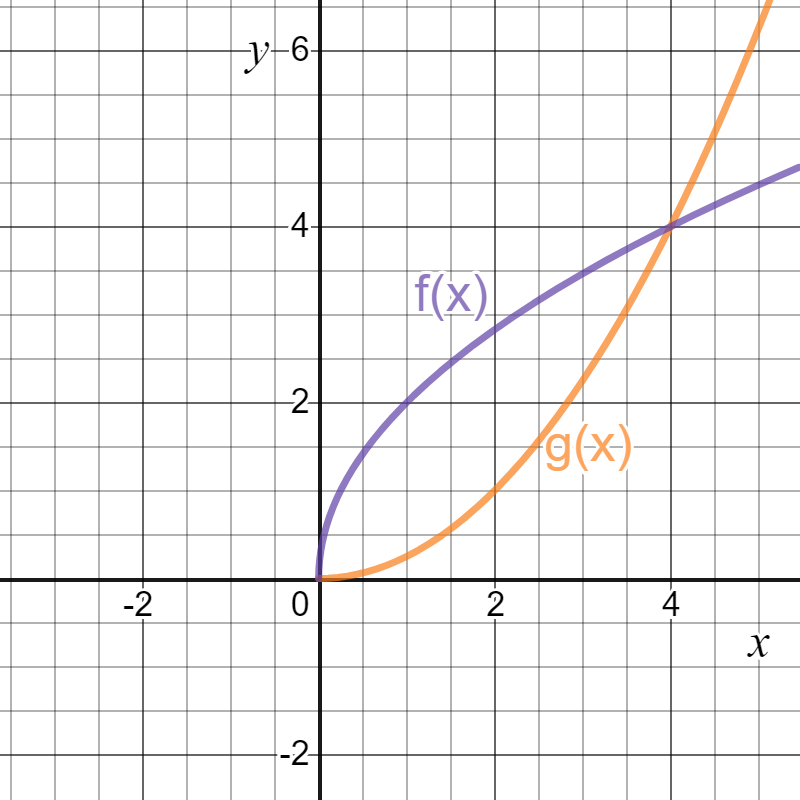
\includegraphics[width=0.8\textwidth]{img/desmos-two-functions.png}

\end{exercise}

